\documentclass[Nike]{tuberlinbeamer}
\graphicspath{{./tuberlinbeamer/}{./figures/}{./../scripts/figures}}
\usepackage[english]{babel}  % 'babel' muss geladen werden
\usepackage[utf8]{inputenc}  % optional, aber empfehlenswert
\usepackage{amsmath,amssymb}
\usepackage{hyperref}
% recommended styles: authoryear, alphabetic
\usepackage[style=authoryear]{biblatex}

\bibliography{references.bib}
\setbeamertemplate{bibliography item}{}
% Use Chancery Font
\DeclareMathAlphabet{\mathpzc}{OT1}{pzc}{m}{it}

\usepackage{subfig}
\usepackage{hyperref}
\usepackage{svg}
\usepackage{algorithm2e}

%\usepackage{showframe}

\newcommand{\x}{\boldsymbol{x}}
\newcommand{\y}{\boldsymbol{y}}


% Notes on second screen (\note{...}) using `pdfpc --notes=right generative_nns.pdf`.
%\usepackage{pgfpages}
%\usepackage{mybeamerbasenotes}
%\setbeameroption{show notes on second screen}

\title{Unsupervised Learning}
\author{Malte Esders, Christopher Anders, Wojciech Samek}
\institute{Technische Universität Berlin - Machine Learning Group}

% Eigenes Logo einfuegen:
\renewcommand{\pathtomylogo}{ida_logo}

\usepackage{mycommands}

\AtBeginSection[]
{
  \begin{frame}
    \frametitle{Agenda}
    \setcounter{tocdepth}{1}
    \tableofcontents[currentsection]
  \end{frame}
}

\AtBeginSubsection[]
{
  \begin{frame}
    \frametitle{Agenda}
    \setcounter{tocdepth}{2}
    \tableofcontents[currentsection,currentsubsection]
  \end{frame}
}


%%%%%%%%%%%%%%%%%%%%%%%%%%%%%%%%%%%%%%%%%%%%%%%%%%%%%%%
%%%%%%%%%%%%%%%%%%%%%%%%%%%%%%%%%%%%%%%%%%%%%%%%%%%%%%%
%%%%%%%%%%%%%%%%%%%%%%%%%%%%%%%%%%%%%%%%%%%%%%%%%%%%%%%
\begin{document}


\frame{\titlepage}


\begin{frame}
  \frametitle{This presentation}
  Presentation repository: \\
  \begin{center}
    \url{https://github.com/Maltimore/unsupervised_learning_lecture}\\
  \end{center}
  Contains all code to generate plots\\
  Parts not otherwise marked: BSD licensed
\end{frame}

\begin{frame}
  \frametitle{Agenda}
  \setcounter{tocdepth}{1}
  \tableofcontents
\end{frame}


\section{Introduction and intuition}
\subsection{Unsupervised Learning}

\begin{frame}
 \frametitle{Unsupervised Learning}
  \begin{center}
    \vfill
    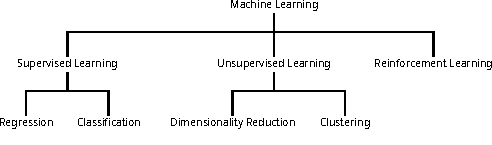
\includegraphics[width=\textwidth]{ml_schema}
    \vfill
  \end{center}
\end{frame}

\begin{frame}
 \frametitle{Unsupervised Learning}
  \begin{center}
    \vfill
    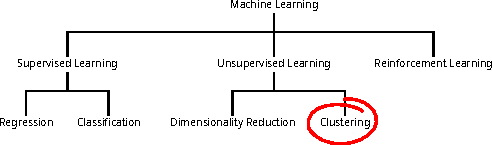
\includegraphics[width=\textwidth]{ml_schema_sel}
    \vfill
  \end{center}
\end{frame}

\begin{frame}
 \frametitle{Unsupervised Learning}
  \begin{center}
    \begin{quote}
      When we’re learning to see, nobody's telling us what the right
      answers are - we just look. Every so often, your mother says
      ’that's a dog’, but that's very little information. You'd be lucky if
      you got a few bits of information - even one bit per second - that
      way. The brain's visual system has $10^{14}$ neural connections. And
      you only live for $10^9$ seconds. So it's no use learning one bit per
      second. You need more like $10^5$ bits per second. And there's only
      one place you can get that much information: from the input
      itself.
    \end{quote}
  Geoffrey Hinton, 1996
  \end{center}
  Genome: $3 * 10^9$ base-pairs (A, T, C, G), with 2 bits per location has  $6 * 10^9$ bits.
\end{frame}


\subsection{Cluster examples}
\begin{frame}
 \frametitle{Clusters - Intuition}
  \begin{center}
    Without labels:
    \centering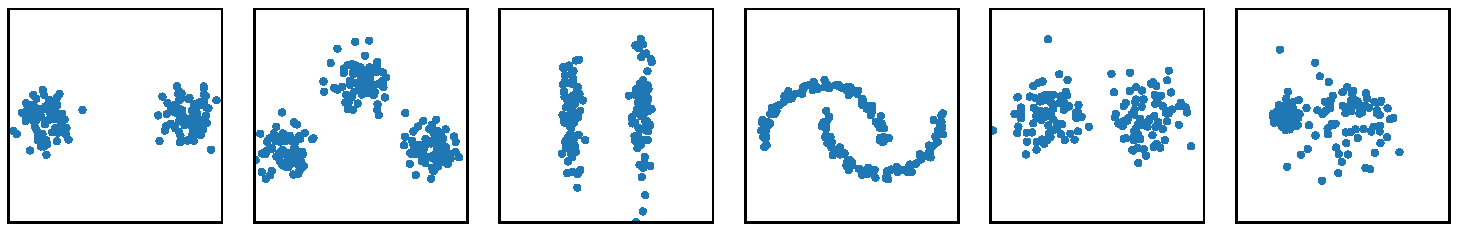
\includegraphics[width=1.0\textwidth]{sample_clusters.pdf}
    \pause
    ``True'' clusters:
    \centering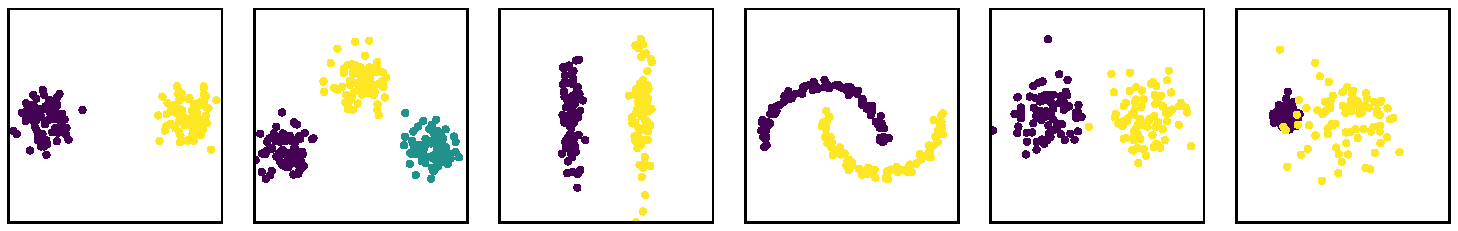
\includegraphics[width=1.0\textwidth]{sample_clusters_true_assignment.pdf}
  \end{center}
  We do not have the ``true'' clusters with real data!
\end{frame}

\begin{frame}
 \frametitle{Clusters - Intuition}
  Clustering is an ill-posed problem: no definition of a cluster.\\
  Some approaches:
  \begin{itemize}
    \item samples within a cluster should be ``similar'', samples between clusters ``different''
    \item clusters are regions of densely populated feature space
    \item samples in the same cluster come from the same underlying process
  \end{itemize}
\end{frame}


\section{Distance and Similarity measures}
\subsection{Euclidean distance}
\begin{frame}[t]
  \frametitle{Euclidean distance}
  \begin{columns}[T]
    \onslide
    \column{0.6\textwidth}
      Pythagoras formula:
      \begin{align*}
        c^2 &= a^2 + b^2\\
        c   &= \sqrt{a^2 + b^2}
      \end{align*}
      \pause
      Euclidean distance notation:
      \begin{equation*}
        d(\x, \y)= \sqrt{\Delta x_1^2 + \Delta x_2^2}
      \end{equation*}
      \only<3-5>{\
        Euclidean distance 3-D:\
        \begin{align*}\
          \overline{BC} &= \sqrt{\overline{AC}^2 + \overline{AB}^2}\\
          \only<4>{\
            \overline{BD} &= \sqrt{\overline{BC}^2 + \overline{CD}^2}\
          }\
          \only<5>{\
            \overline{BD} &= \sqrt{\overline{AC}^2 + \overline{AB}^2 + \overline{CD}^2}\
          }\
        \end{align*}\
      }
      \only<6->{\
        Euclidean distance d-D:\
        \begin{equation*}\
          d(\x, \y) = \sqrt{\sum_{i=1}^d \Delta x_i^2}\
        \end{equation*}\
      }
    \column{0.3\textwidth}
      \onslide<1->
      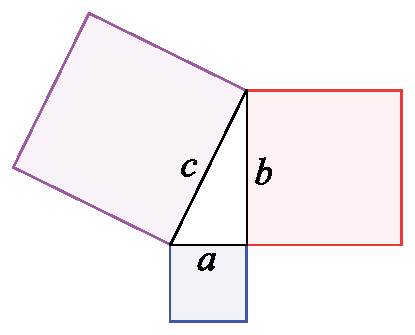
\includegraphics[width=.8\textwidth]{pythagoras.pdf}
      \tiny Wikipedia Pythagorean theorem
      \vskip 2mm
      \onslide<3->
      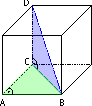
\includegraphics[width=.7\textwidth]{ndeuclidean.pdf}
  \end{columns}
\end{frame}

\begin{frame}[t]
  \frametitle{Manhattan distance}
  \begin{columns}[T]
    \column{0.6\textwidth}
      ``Manhattan'' / ``Taxicab'' distance
      \begin{equation*}
        d(\x, \y) = \sum_{i=1}^d |\Delta x_i|
      \end{equation*}
      Usage: LASSO regularization
    \column{0.3\textwidth}
      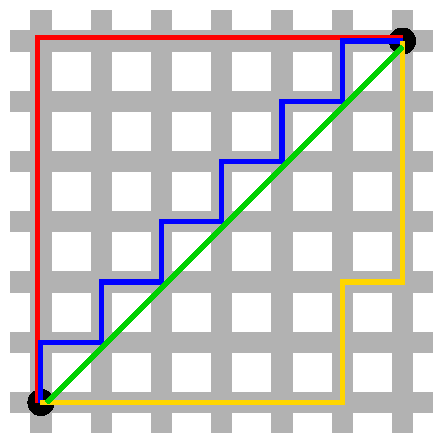
\includegraphics[width=\textwidth]{manhattan.pdf}
      \tiny Wikipedia Manhattan distance
  \end{columns}
\end{frame}

\subsection{Minkowski distance}
\begin{frame}[t]
  \frametitle{Minkowski distance}
  \begin{columns}[T]
    \column{0.6\textwidth}
      Minkowski distance generalizes Euclidean and Manhattan distance:
      \todo{Notation $\Delta x_i$ is confusion because x is used already.}
      \begin{equation*}
        d(\x, \y) = \Bigg(\sum_{i=1}^d |\Delta x_i|^p\Bigg)^{1/p}
      \end{equation*}
      \pause
      $p=1$: Manhattan distance\\
      $p=2$: Euclidean distance\\
      \pause
      $p=\infty$:
      \begin{equation*}
        d(\x, \y) = \max_{i} |\Delta x_i|
      \end{equation*}
      \pause
      $p\rightarrow0$:
      \begin{equation*}
        d(\x, \y) = \min_{i} |\Delta x_i|
      \end{equation*}
      \pause
    \column{0.3\textwidth}
      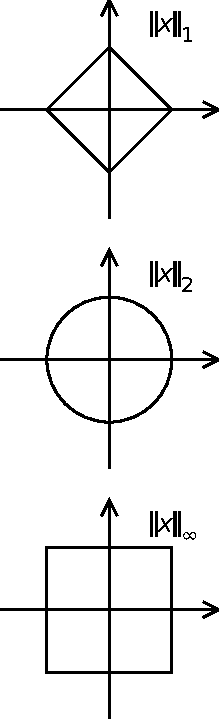
\includegraphics[width=0.5\textwidth]{minkowski_norms.pdf}\\
      \tiny Wikipedia Norm (mathematics)
  \end{columns}
\end{frame}

\subsection{Vector norm notation}
\begin{frame}
  \frametitle{Vector norm}
  The distance between vectors is the vector-norm of their difference:
  \begin{equation*}
    d(\x, \y) = \Bigg(\sum_{i=1}^d |\Delta x_i|^p\Bigg)^{1/p} = ||\x - \y||_p
  \end{equation*}
  \pause
  For $p=2$, the shorthand is:
  \begin{equation*}
    ||\x - \y||_2 = ||\x - \y||
  \end{equation*}
\end{frame}


\subsection{Squared euclidean distance}
\begin{frame}
  \frametitle{Squared euclidean distance}
  Squared euclidean distance:
  \begin{equation*}
    ||\x - \y||_2^2 = \sum_{i=1}^d |\Delta x_i|^2
  \end{equation*}
  \pause
  Do not confuse
  \begin{equation*}
    ||\x - \y|| = ||\x - \y||_2 \neq ||\x - \y||^2 = ||\x - \y||_2^2
  \end{equation*}
  \pause
  Squared Euclidean distance:
  \begin{itemize}
    \item not a true metric (no triangle inequality)
    \item overemphasizes big distances (and vice versa)
    \item makes some optimization problems converge better
  \end{itemize}
\end{frame}

\subsection{Cosine distance}
\begin{frame}[t]
  \frametitle{Cosine distance}
  \begin{columns}[T]
    \column{0.45\textwidth}\
    Cosine distance only compares angles between vectors.\\\
    \uncover<2->{\
      Cosine definition:\
      \begin{align*}\
        \x^\intercal \y &= |\x||\y|cos(\alpha)\\ \
        cos(\alpha) &= \frac{\x^\intercal \y}{|\x||\y|} \
      \end{align*}\
    }\
    \uncover<3->{\
      Cosine distance:\
      \begin{equation*}\
        d(\x, \y) = 1 - \frac{\x^\intercal \y}{|\x||\y|}\
      \end{equation*}\
    }\
    \column{0.45\textwidth}
    \only<1-3>{\
      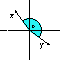
\includegraphics[width=.8\textwidth]{cosine_distance}\
    }\
  \end{columns}
\end{frame}

\subsection{Z-scores}
\begin{frame}
  \frametitle{Different scales}
  Measurements can be at different scales (for instance cm, kg etc.)\\
  We can normalize:
  \begin{equation*}
    z = \frac{x - \mu}{\sigma}
  \end{equation*}
  \pause
  \centering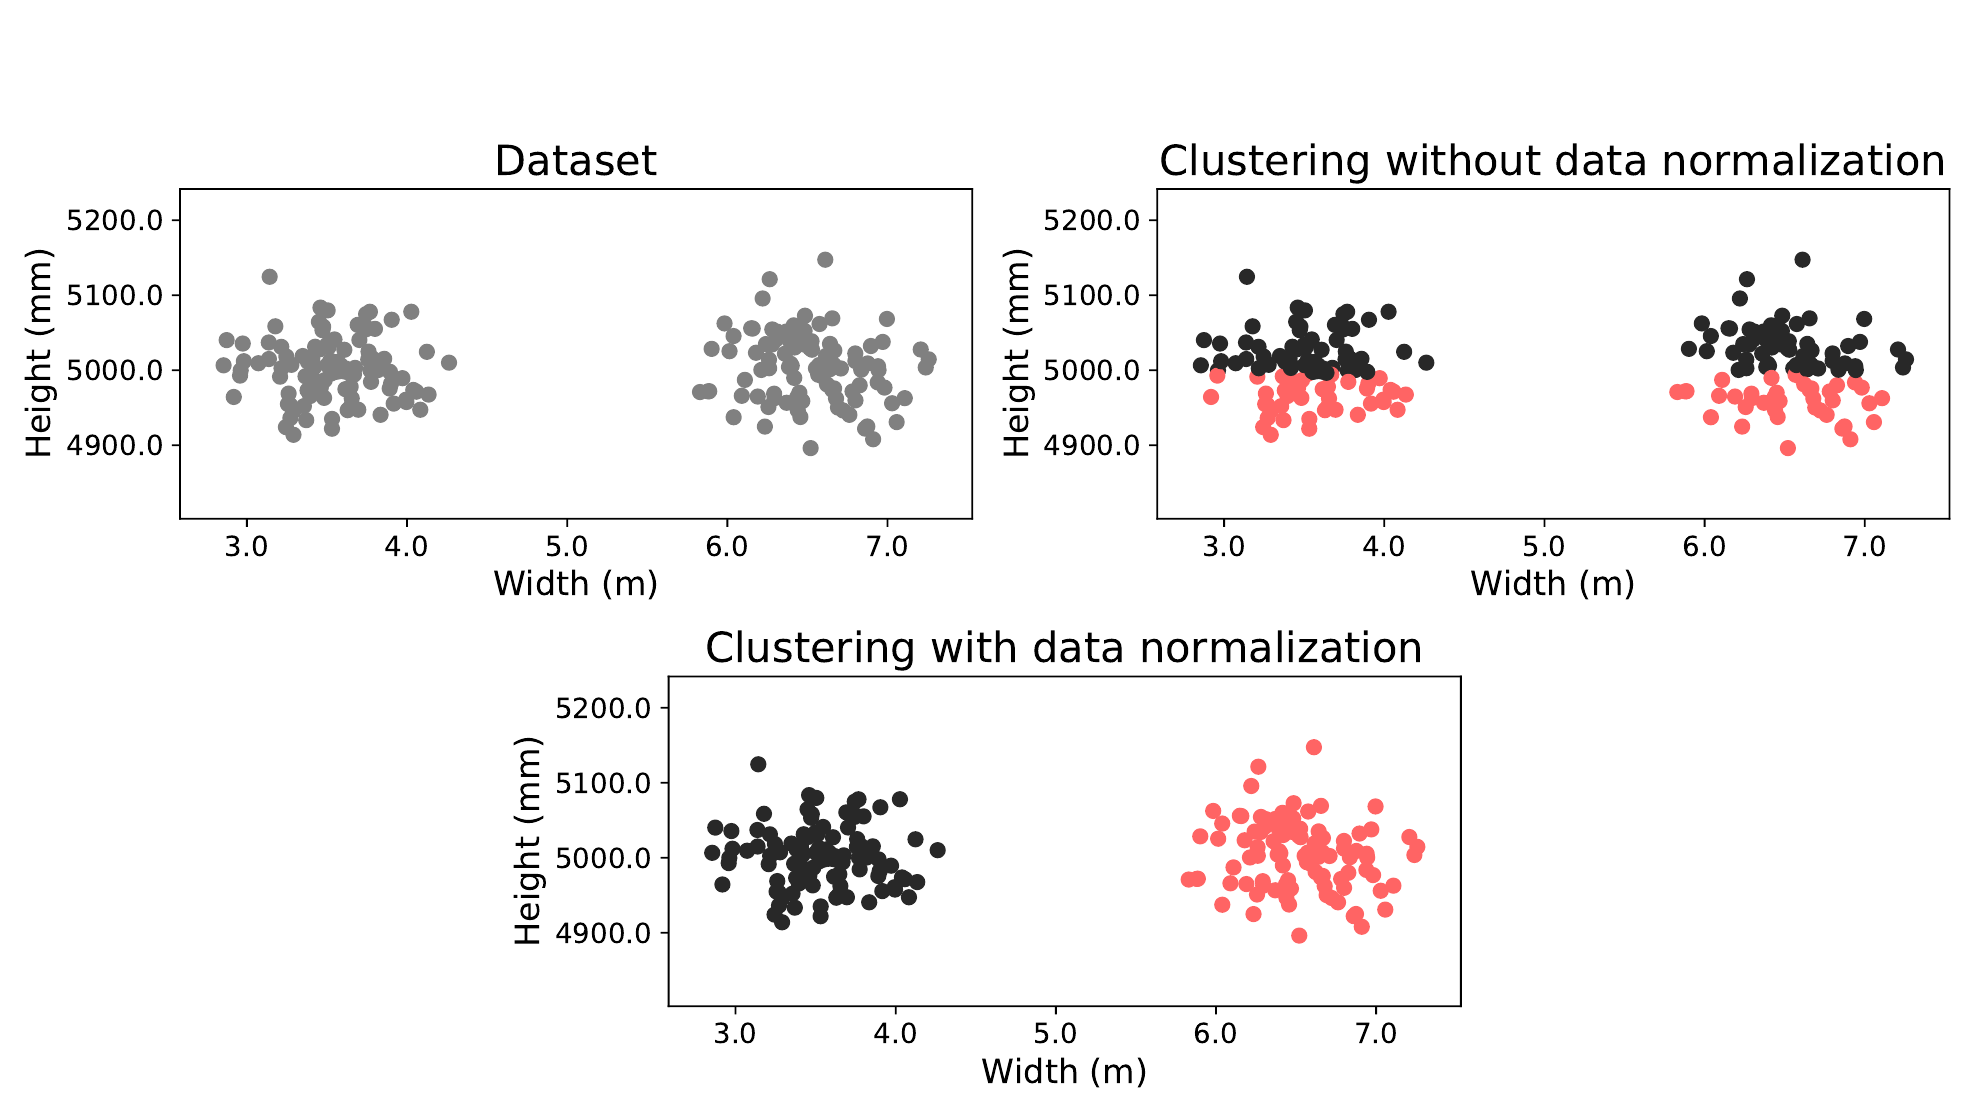
\includegraphics[width=0.7\textwidth]{normalization_clustering.png}
  \tiny \cite{guerin_clustering_2017}
\end{frame}


\section{Clustering algorithms}
\begin{frame}
  \vfill
  \centering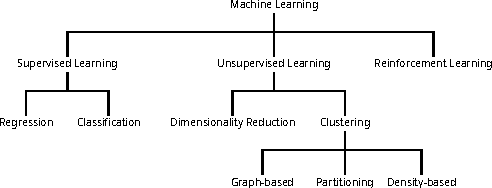
\includegraphics[width=\textwidth]{ml_schema_ext}
  \vfill
\end{frame}

\subsection{Hierarchical Clustering}
\begin{frame}
  \frametitle{Hierarchical Clustering}
  \begin{itemize}[<+->]
    \item graph-based
    \item builds a hierarchy of clusters, either top down (``divisive'') or bottom up (``agglomerative'')
    \item intuitive
    \item suggests numbers of clusters
    \item arbitrary cluster shapes
    \item sensitive to noise
  \end{itemize}
\end{frame}

\begin{frame}
  \frametitle{Agglomerative clustering algorithm:}
  Let $\mathpzc{D}_i$, $\mathpzc{D}_j$ be the sets containing the samples in clusters $i$ and $j$.  \\
  \bigskip

  choose $n_{final}$ clusters\\
  initialize $\mathpzc{D}_i$ as singleton clusters\\
  initialize $n_{clusters} = n_{samples}$\\
  \While{$n_{clusters} > n_{final}$}{
    find clusters $i$ and $j$ with smallest distance\\
    merge $\mathpzc{D}_i$ and $\mathpzc{D}_j$\\
    $n_{clusters} \leftarrow n_{clusters} - 1$
  }
  return clusters
\end{frame}

\begin{frame}
  \frametitle{Dendrogram with Euclidean distance}
  \begin{center}
    \centering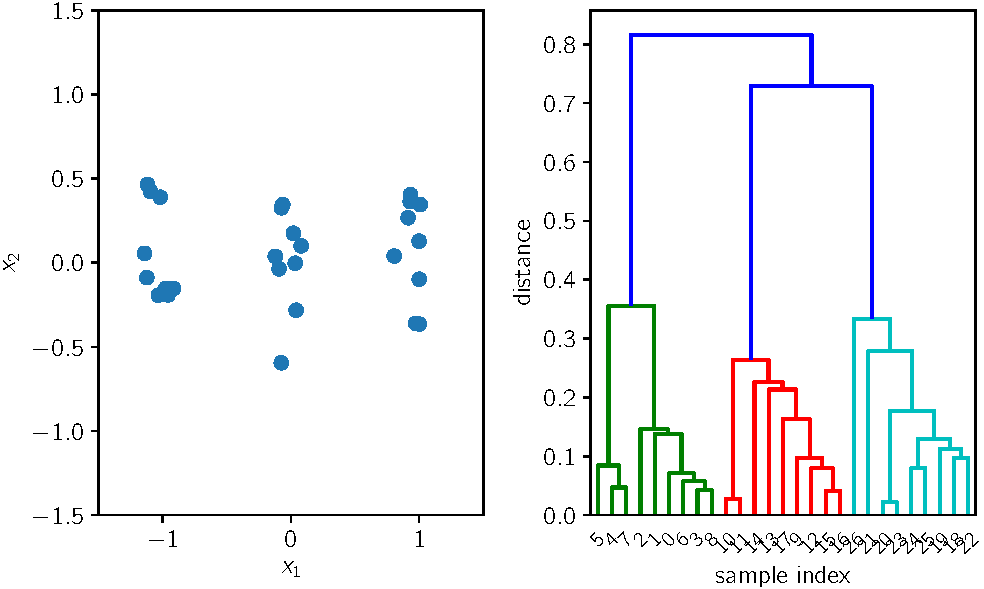
\includegraphics[width=0.8\textwidth]{dendrogram_euclidean.pdf}
  \end{center}
\end{frame}

\begin{frame}
  \frametitle{Dendrogram with squared Euclidean distance}
  \begin{center}
    \centering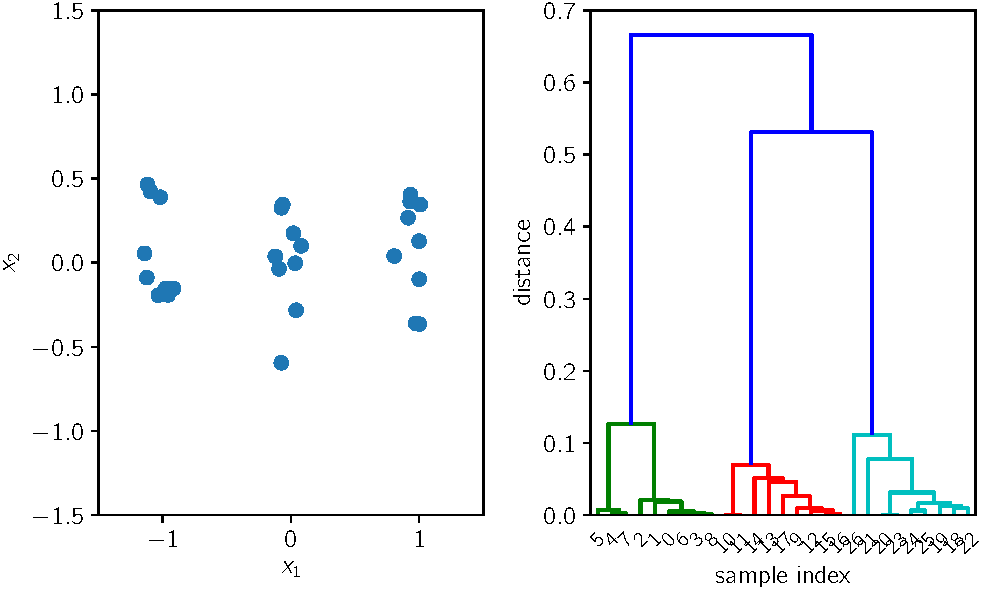
\includegraphics[width=0.8\textwidth]{dendrogram_squared_euclidean.pdf}
  \end{center}
\end{frame}


\begin{frame}
  \frametitle{Cluster distance measures}
  Let $\mathpzc{D}_i$, $\mathpzc{D}_j$ be the sets containing the samples in clusters $i$ and $j$.
  \\
  Minimum linkage:
  \begin{equation*}
    d_{min}(\mathpzc{D}_i, \mathpzc{D}_j) = \min_{\x \in \mathpzc{D}_i, \x' \in \mathpzc{D}_j} ||\x - \x'||
  \end{equation*}
  \pause
  \\
  Maximum or ``complete'' linkage:
  \begin{equation*}
    d_{max}(\mathpzc{D}_i, \mathpzc{D}_j) = \max_{\x \in \mathpzc{D}_i, \x' \in \mathpzc{D}_j} ||\x - \x'||
  \end{equation*}
  \\
  \pause
  Average linkage:
  \begin{equation*}
    d_{avg}(\mathpzc{D}_i, \mathpzc{D}_j) = \frac{1}{n_i n_j} \sum_{\x \in \mathpzc{D}_i} \sum_{\x' \in \mathpzc{D}_j} ||\x - \x'||
  \end{equation*}
  \scriptsize Notation from \cite{duda2012pattern}
\end{frame}

\begin{frame}
  \frametitle{Original data}
  After clustering, assignments can seem ``natural'', good to compare original data:
  \begin{center}
    \centering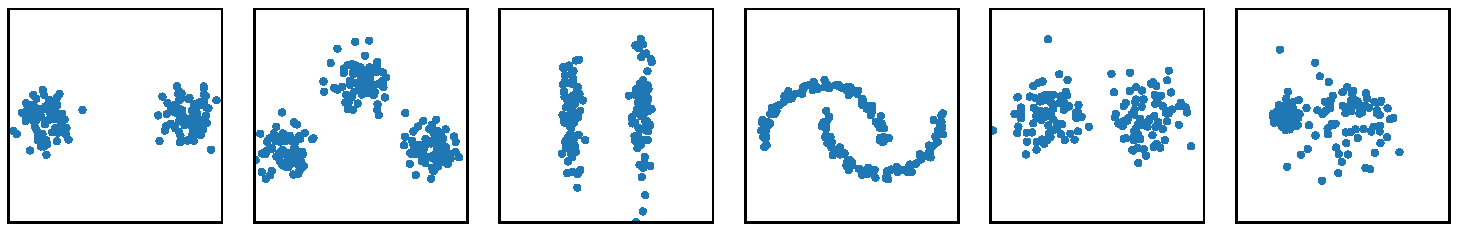
\includegraphics[width=0.95\textwidth]{sample_clusters.pdf}
  \end{center}
\end{frame}

\begin{frame}
  \frametitle{Agglomerative clustering results}
  \begin{center}
    \scriptsize Minimum
    \centering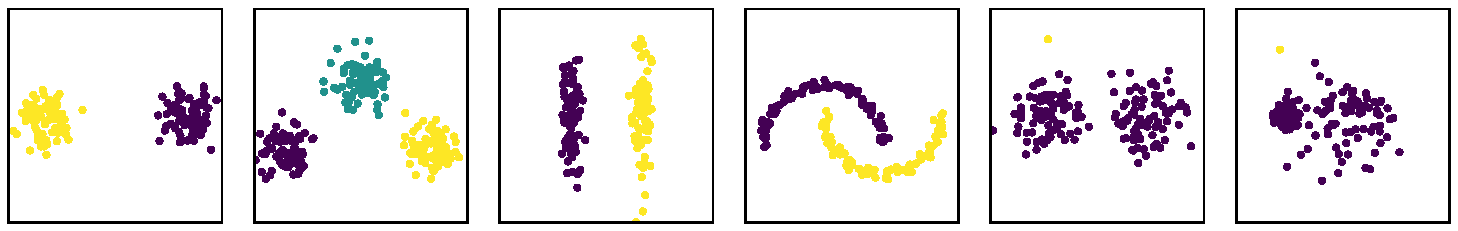
\includegraphics[width=0.95\textwidth]{agglomerative_clusters_minimum_linkage.pdf}
    \pause
    \scriptsize Maximum
    \centering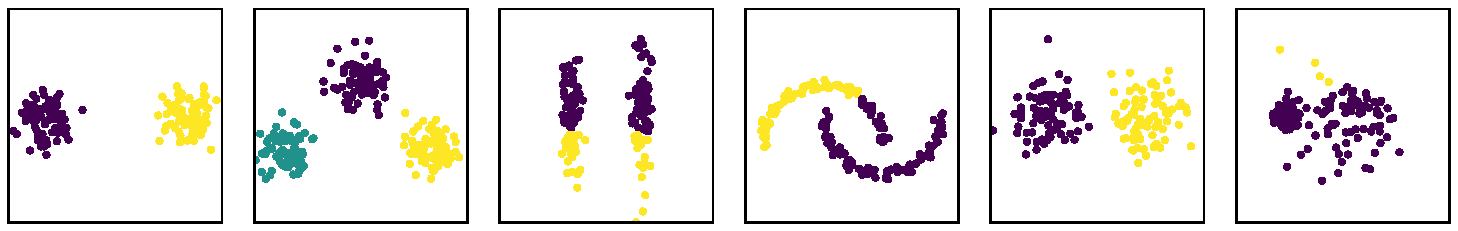
\includegraphics[width=0.95\textwidth]{agglomerative_clusters_complete_linkage.pdf}
    \pause
    \scriptsize Average
    \centering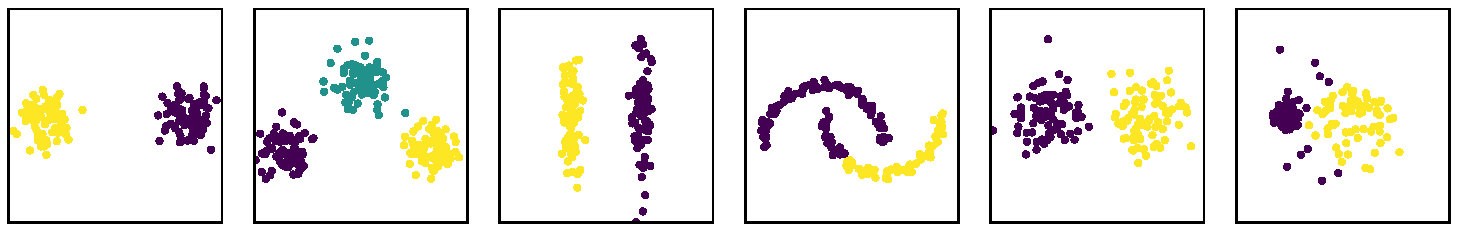
\includegraphics[width=0.95\textwidth]{agglomerative_clusters_average_linkage.pdf}
  \end{center}
\end{frame}

\begin{frame}
  \frametitle{Tips and tricks}
  \begin{center}
   \centering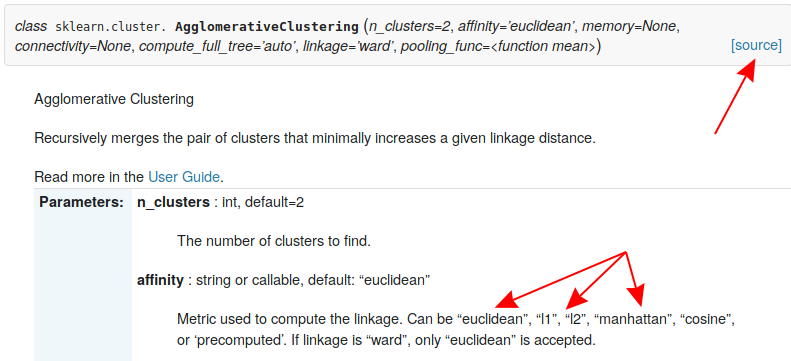
\includegraphics[width=0.90\textwidth]{sklearn_API_doc.png}
  \end{center}
  Sometimes, documentation can be confusing:
  \\
  What is the difference between ``l2'' and ``euclidean''?
  \\
  Or ``l1'' and ``manhattan''?
\end{frame}


\begin{frame}
  \frametitle{Tips and tricks}
  Looking into the code:
  \begin{center}
    \centering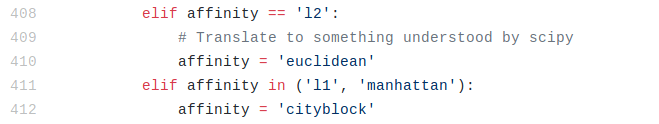
\includegraphics[width=0.95\textwidth]{sklearn_code.png}
  \end{center}
  In the background it does exactly the same.
\end{frame}

\subsection{K-Means}
\begin{frame}
  \frametitle{K-Means}
  Idea: prototype for every cluster
  \\
  Prototype is mean of all samples in cluster $c$, $\mathpzc{D}_c$:
  \begin{equation*}
    \mu_c = \frac{1}{n_c} \sum_{i \in \mathpzc{D}_c} x_i
  \end{equation*}
  \pause
  Minimize distance from prototype to each member in the cluster:
  \begin{equation*}
    \mathpzc{L} = \sum_c \sum_{i \in \mathpzc{D}_c} d(\x_i, \mu_c)
  \end{equation*}
  \pause
  Finding a solution is NP-hard
  \\
  K-means cannot work with pairwise data such as user ratings
\end{frame}


\begin{frame}
  \frametitle{K-Means algorithm}
  initialize $\mu_c$ to random samples\\
  \While{clusters change}{
    assign $\mu_c$\ to cluster means\\
    assign samples to clusters\\
  }
  return clusters
\end{frame}


\begin{frame}
  \frametitle{K-Means clusters}
  \begin{center}
    K-Means assignment:
    \centering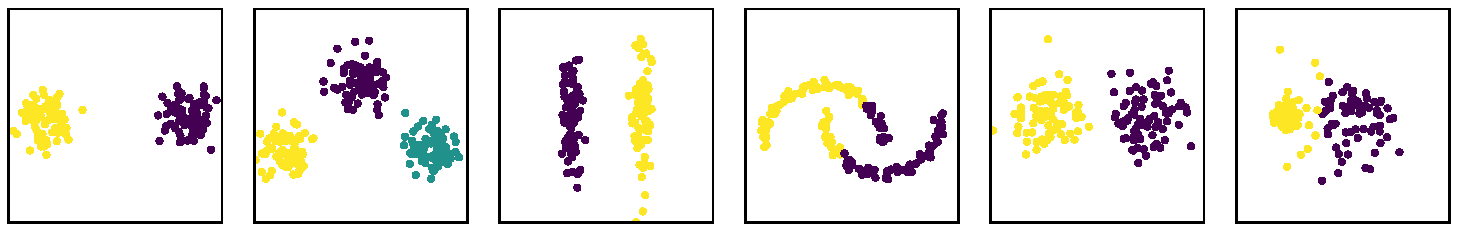
\includegraphics[width=1.0\textwidth]{kmeans_clusters.pdf}
    \pause
    Voronoi tesselation:
    \centering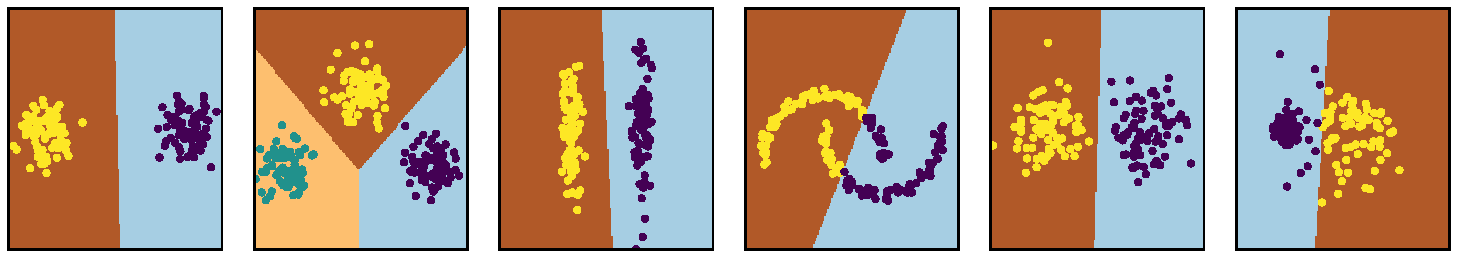
\includegraphics[width=1.0\textwidth]{kmeans_clusters_voronoi.pdf}
  \end{center}
  Voronoi diagram not possible with hierarchical clustering!
\end{frame}

\subsection{DBSCAN}
\begin{frame}
  \frametitle{DBSCAN}
  \begin{itemize}
    \item clusters are regions of high density separated by regions of low density
    \item arbitrary cluster shapes
  \end{itemize}
  \begin{centering}
  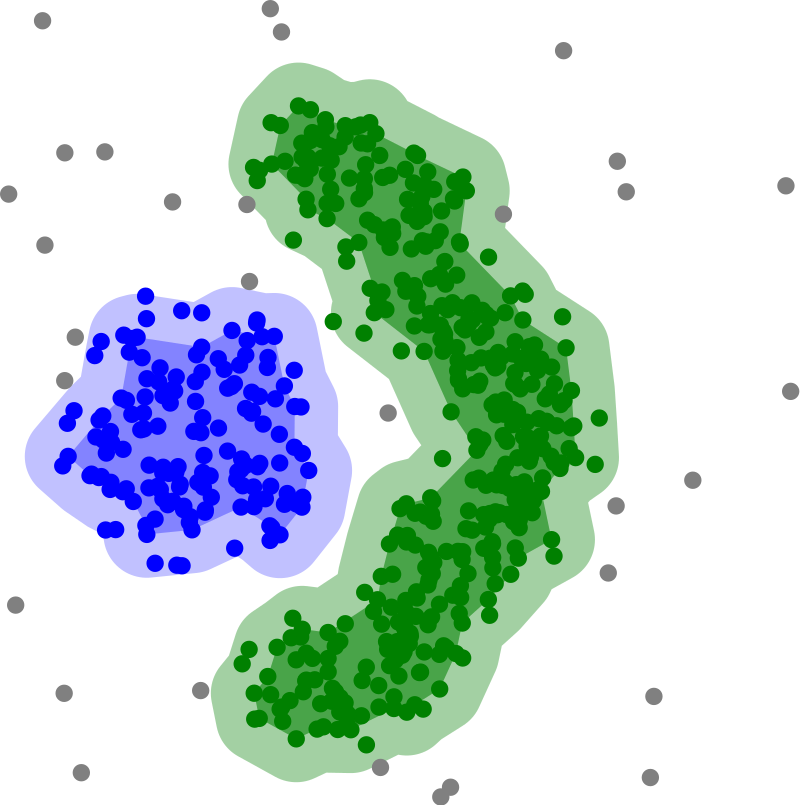
\includegraphics[width=0.5\textwidth]{DBSCAN_data.png}
  \tiny \cite{ester1996density}\\
  \end{centering}
  \pause
  \normalsize
  \begin{itemize}
    \item very simple, but effective (2014 SIGKDD test-of-time award (\cite{schubert2017dbscan}))\\
    \item explicit noise point modeling
  \end{itemize}
\end{frame}

\begin{frame}
  \frametitle{DBSCAN}
  \begin{columns}[T]
    \column{0.6\textwidth}
      \onslide<1->
       Two parameters:
       \begin{itemize}
         \item $\epsilon$: distance, defines a neighborhood
         \item MinPts: amount of neighbors to be a core point
       \end{itemize}
       \pause
      Three types of points:
      \begin{itemize}
        \item core
        \item border
        \item noise
      \end{itemize}
    \column{0.3\textwidth}
      \onslide<3->
      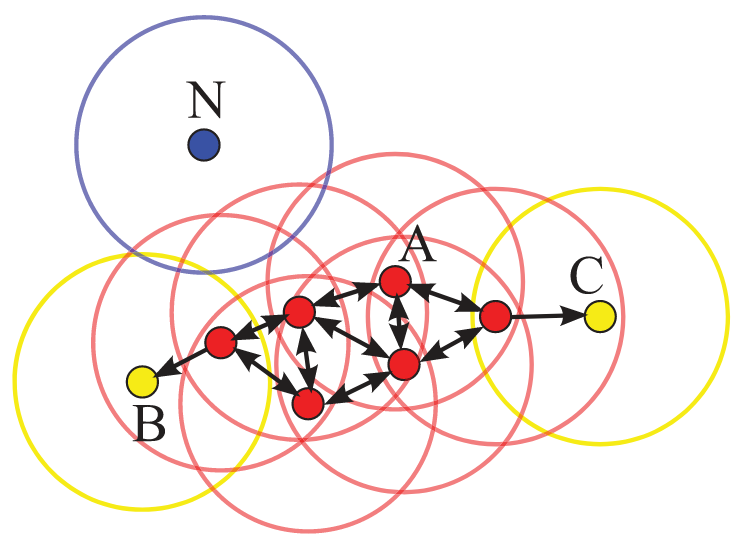
\includegraphics[width=1.0\textwidth]{DBSCAN_illustration.png}\\
      \tiny \cite{schubert2017dbscan}
  \end{columns}
\end{frame}


\begin{frame}
  \frametitle{DBSCAN clustering results}
  \begin{center}
    \scriptsize $\epsilon = 0.1$, MinPts $=4$
    \centering\includegraphics[width=0.95\textwidth]{{DBSCAN_clusters_eps_0.1_MinPts_4}.pdf}
    \pause
    \scriptsize $\epsilon = 0.2$, MinPts $=4$
    \centering\includegraphics[width=0.95\textwidth]{{DBSCAN_clusters_eps_0.2_MinPts_4}.pdf}
    \pause
    \scriptsize $\epsilon = 0.2$, MinPts $=20$
    \centering\includegraphics[width=0.95\textwidth]{{DBSCAN_clusters_eps_0.2_MinPts_20}.pdf}
  \end{center}
\end{frame}


\subsection{More examples}
\begin{frame}
  \frametitle{Overview of clustering algorithms}
  \begin{center}
    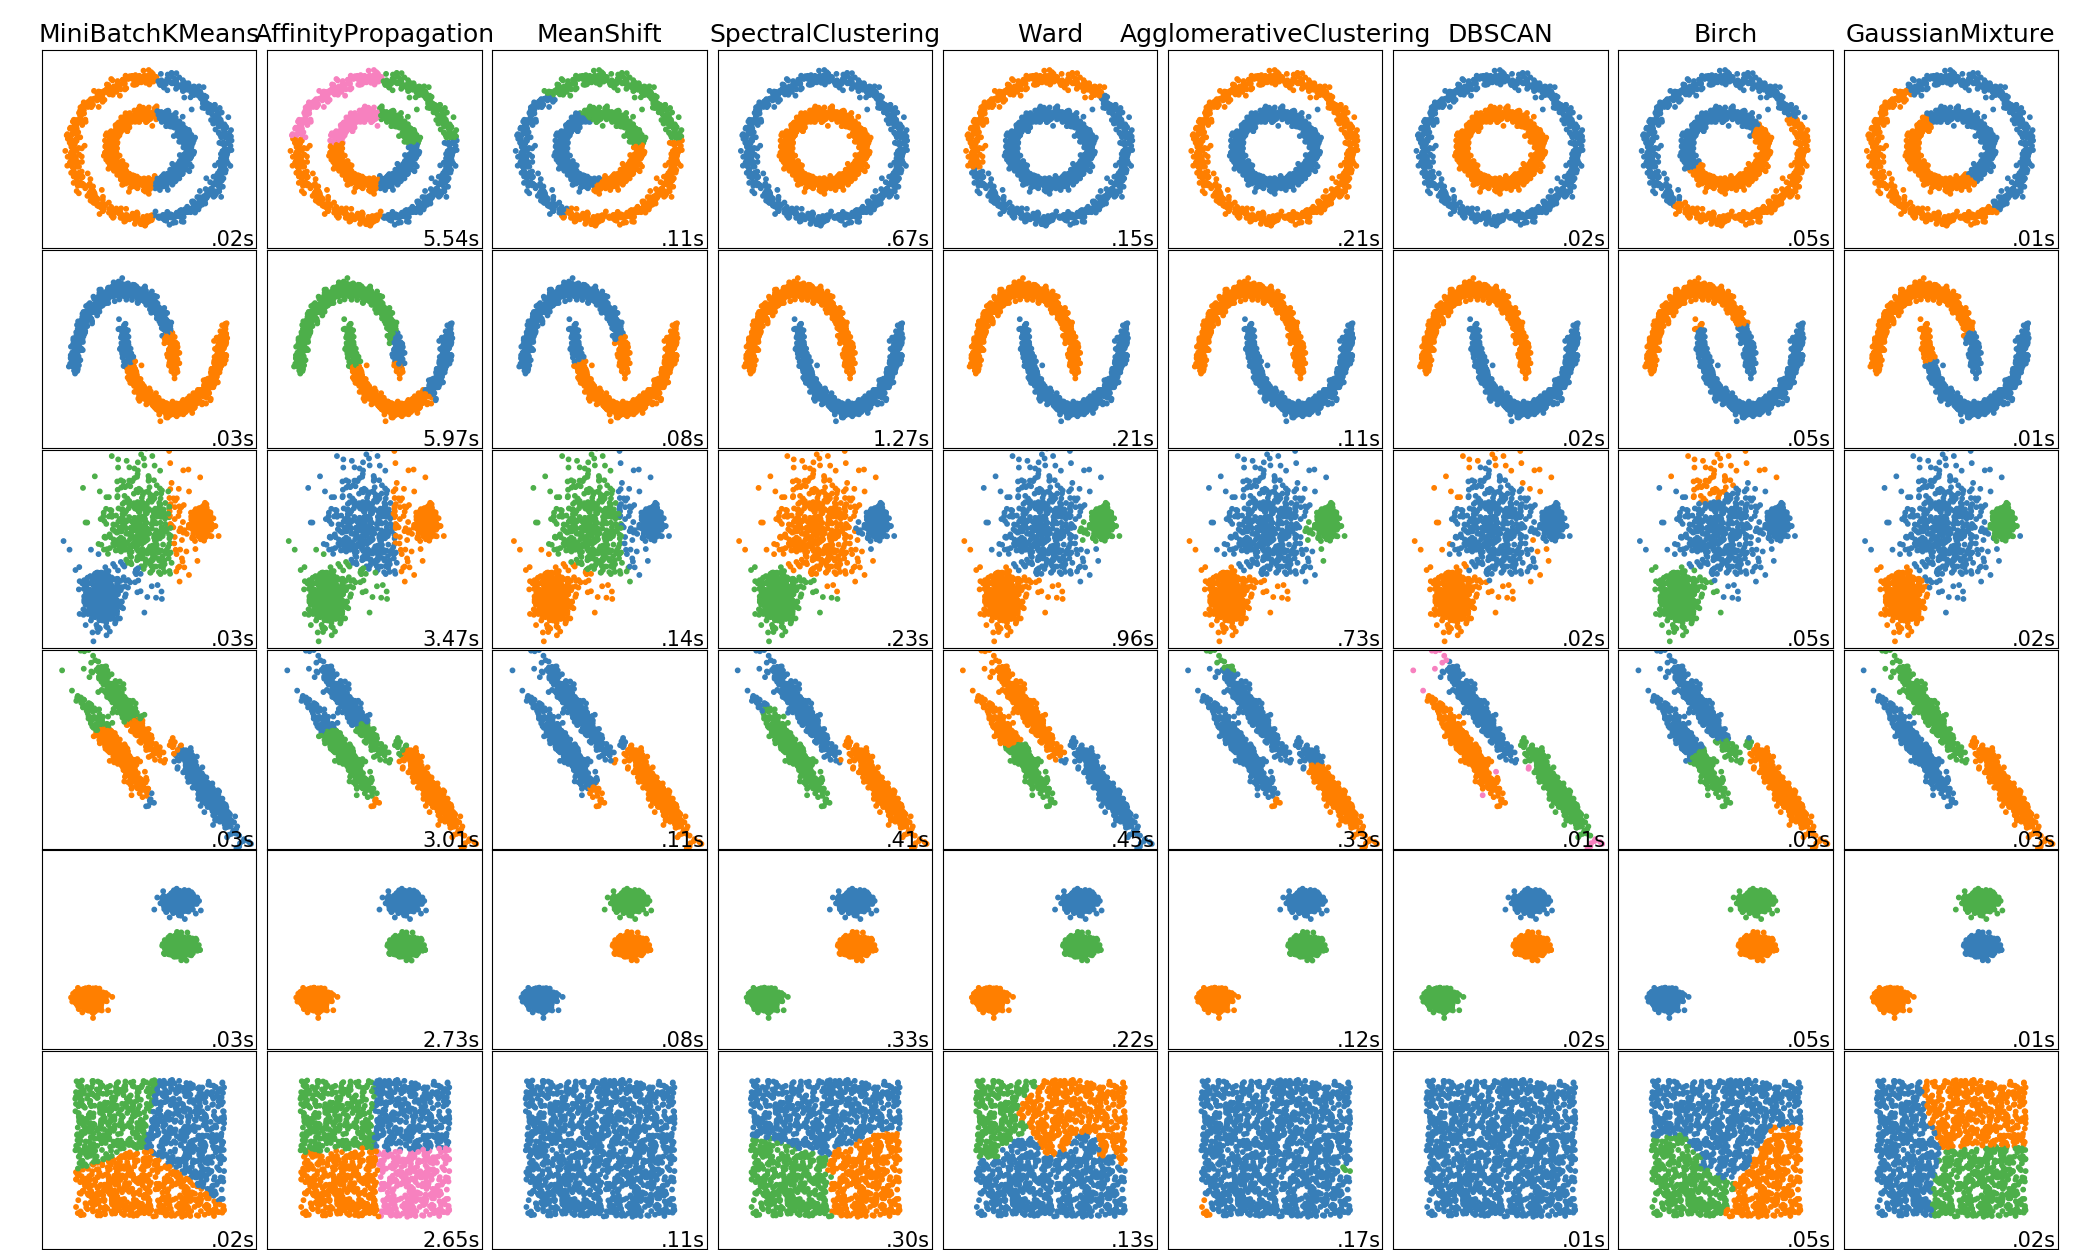
\includegraphics[width=0.85\textwidth]{sklearn_doc_examples.png}
  \end{center}
  \tiny \url{http://scikit-learn.org/stable/modules/clustering.html} \cite{pedregosa2011scikit}
\end{frame}


\begin{frame}%[allowframebreaks]  % Uncomment if you need more than one page for references
  \frametitle{References}
  \printbibliography
\end{frame}

\end{document}
